\documentclass[a4paper, 10pt, french]{article}
% Préambule; packages qui peuvent être utiles
   \RequirePackage[T1]{fontenc}        % Ce package pourrit les pdf...
   \RequirePackage{babel,indentfirst}  % Pour les césures correctes,
   % et pour indenter au début de chaque paragraphe
   \RequirePackage[utf8]{inputenc}   % Pour pouvoir utiliser directement les accents
   % et autres caractères français
   % \RequirePackage{lmodern,tgpagella} % Police de caractères
   \textwidth 17cm \textheight 25cm \oddsidemargin -0.24cm % Définition taille de la page
   \evensidemargin -1.24cm \topskip 0cm \headheight -1.5cm % Définition des marges
   % \RequirePackage{latexsym}                  % Symboles
   % \RequirePackage{amsmath}                   % Symboles mathématiques
   % \RequirePackage{tikz}   % Pour faire des schémas
   \RequirePackage{graphicx} % Pour inclure des images
   % \RequirePackage{listings} % pour mettre des listings
   % Fin Préambule; package qui peuvent être utiles

\title{Rapport de TP 4MMAOD : Génération d'ABR optimal}
\author{
	Maxime Deloche \\
	Ludovic Carré \\
	\textit{Equipe Teide 4} \\
	\textbf{2ème partie du rendu}
}

\begin{document}

\maketitle

% \section{Equation de Bellman}
%
% \subsection{Question 1}
%
% \subsubsection{Montrons que tout sous-arbre d'un ABR optimal est un ABR optimal, par l'absurde.}
%
% Soit A un ABR optimal. On suppose qu'un sous-arbre S de A n'est pas optimal.
% Donc le nombre de comparaisons $x$ pour atteindre un élément $e$ de S n'est pas optimal dans S (notons cet optimal $x_{opt}$).
% Donc le nombre de comparaisons pour atteindre $e$ dans A est $x + 1$. Or, on pourrait atteindre $e$ en $x_{opt} + 1$, donc A n'est pas optimal, ce qui est absurde. \\
%
% Donc tout sous-arbre d'un ABR optimal est un ABR optimal.
%
%
% \subsubsection{Equation de Bellman}
%
% Deux raisonnements différents nous ont conduit à deux équations de Bellman différentes mais équivalentes. Nous les avons implémentées et on obtient des résultats identiques et corrects.\\
% \begin{itemize}
% 	\item[$\bullet$] \textbf{Version 1} \\
% 		Dans un arbre A de racine $e_i$, on a :
% 		\begin{itemize}
% 			\item[$\bullet$] une probabilité \verb?proba_que_element_soit_e_i? de faire 1 comparaison (si l'élément cherché est $e_i$).
% 			\item[$\bullet$] une probabilité \verb?proba_que_element_soit_dans_le_sous_arbre_gauche? de faire le nombre de comparaisons optimal du sous-arbre gauche, plus 1.
% 			\item[$\bullet$] une probabilité \verb?proba_que_element_soit_dans_le_sous_arbre_droit? de faire le nombre de comparaisons optimal du sous-arbre droit, plus 1.
% 		\end{itemize}
%
% 		Soit $c(E)$ le nombre de comparaisons moyen optimal de l'arbre formé par les éléments de E. L'équation de Bellman est : 
% 		\[ C(E) = \min_{e_i \in E} ( \frac{p_i}{\sum\limits_{e_l \in E}{p_l}} + \frac{C(\{e_j < e_i\}) + 1}{\sum\limits_{e_l \in E}{p_l}} \sum_{e_j < e_i}{p_j} + \frac{C(\{e_k > e_i\}) + 1}{\sum\limits_{e_l \in E}{p_l}} \sum_{e_k > e_i}{p_k} ) \]
% 		C'est-à-dire : 
% 		\[ C(E) = \min_{e_i \in E} ( 1 + \frac{C(\{e_j < e_i\})}{\sum\limits_{e_l \in E}{p_l}} \sum_{e_j < e_i}{p_j} + \frac{C(\{e_k > e_i\})}{\sum\limits_{e_l \in E}{p_l}} \sum_{e_k > e_i}{p_k} ) \]
% 		Conditions initiales : 
% 		\begin{itemize}
% 			\item $C(E) = 1$ si E ne contient qu'un élément (on ne fait alors qu'une comparaison).
% 			\item $C(E) = 0$ si E est vide. \\
% 		\end{itemize}
%
% 	\item[$\bullet$] \textbf{Version 2} \\
% 		En transformant la formule donnée de calcul du nombre de comparaison moyen optimal en version récursive : 
% 		Soit P la profondeur, initialisée à 1.
% 		L'équation de Bellman est : 
% 		\[ C(E, P) = \min_{e_i \in E} ( p_i.P + C(\{e_j < e_i\}, P+1) + C(\{e_k > e_i\}, P+1) )\]
% 		Conditions initiales : 
% 		\begin{itemize}
% 			\item $C(E) = p_i.P$ si $E = {e_i}$.
% 			\item $C(E) = 0$ si E est vide. \\
% 		\end{itemize}
%
% \end{itemize}
%
%
%
%
% \subsection{Question 2}
%
% \begin{itemize}
% 	\item[$\bullet$] \textbf{Coût de la version 1}
% 		\begin{itemize}
% 			\item \textbf{En mémoire} : on stocke dans un tableau de taille $n$ par $n$ le nombre moyen optimal de comparaisons, ainsi que le noeud choisi en racine pour cet arbre. 
% 				Par exemple, la position $(i, j)$ de ce tableau contiendra le nombre de comparaisons et la racine de l'abre formé par les éléments $e_i$ à $e_j$ 
% 				(en supposant les $e_i$ ordonnés). On a donc un coût en mémoire de $\theta(n^2)$. \\
% 			\item \textbf{En temps} : Pour chaque appel, on a de l'ordre de $k^2$ opérations à effectuer, avec $k$ le nombre d'éléments de E.
% 				On remarque qu'on a $(n - k)$ appels avec $k$ éléments, donc le coût est $\sum\limits_{k=0}^{n} (n-k)k^2 = \frac{1}{12}n(n+1)(n^2+3n+2)$.
% 				On a donc un coût en $\theta(n^4)$. \\
% 		\end{itemize}
% 	\item[$\bullet$] \textbf{Coût de la version 2}
% 		\begin{itemize}
% 			\item \textbf{En mémoire} : On a le même coût en mémoire qu'à la version 1 puisque la valeur optimale ne dépend pas de la profondeur. On est donc en $\theta(n^2)$.
% 			\item \textbf{En temps} : Pour un seul appel, on a un coût en $\theta(1)$ et puisque l'on a $n^2$ appels, on a un coût total de l'ordre de $\theta(n^2)$.\\
% 		\end{itemize}
% \end{itemize}
% \textbf{Conclusion} : On retient donc l'équation de la version 2 puisque elle propose une complexité plus avantageuse.
%
% \newpage
%

%%%%%%%%%%%%%%%%%%%%%%%%%%%%%%%%%%%%%%%%%%%%%%
\section{Principe de notre  programme (1 point)}
{Nous avons implémenté les 2 méthodes (récursive et itérative) pour le calcul du nombre moyen optimal de comparaisons (fonction \verb?avg_comp_rec et avg_comp_iter? de \verb?averagedepth.c?, appelée par \verb?get_avg?). La version itérative est largement plus rapide, et le code la version récursive est commenté.

	C'est l'implémentation directe de notre première version de la formule de Bellman, à laquelle nous avons ajouté des optimisations détaillées dans la partie suivante (nous nous sommes rendus compte d'erreurs de calcul dans la 2e version de l'équation après le rendu de la 1e partie du rapport).

Une fois la fonction \verb?avg_comp_iter? appelée, la fonction \verb?build_tree? construit, à partir du tableau de mémoïsation, l'arbre optimal, et le renvoit.

Enfin, la fonction \verb?treetoarray? écrit, à partir de cet arbre, le code C attendu sur la sortie standard (et peut au passage afficher la profondeur moyenne de cet arbre optimal, stockée dans l'objet \verb?Tree?).\\


Nous avions commencé par une implémentation en Python. Nous nous sommes cependant vite rendus compte de la difficulté à effectuer le moindre calcul d'optimisation et de la lenteur du langage, et avons donc décidé de passer à du C.
Nous avons tout d'abord fait la version récursive, qui était elle aussi très lente. Nous avons fini par réaliser la version itérative qui surpasse de loin la version récursive (cf. partie Performances ci-dessous).
} 

%%%%%%%%%%%%%%%%%%%%%%%%%%%%%%%%%%%%%%%%%%%%%%
\section{Analyse du coût théorique (2 points)}

 \subsection{Choix d'implémentations}
 \begin{itemize}
	 \item Le tableau \verb?comp_array? est un tableau de mémoïsation : à la position \verb?(i, j)?, il stocke l'indice de la racine choisie pour le sous-arbre formé des noeuds d'indices \verb?i? à \verb?j? (les deux inclus), et le nombre de comparaisons moyen de cet arbre optimal.

		 Nous n'avions pas besoin de stocker l'arbre en entier, seulement la racine : en effet, si on sait que la racine est d'indice \verb?k?, on trouve son fils gauche (resp. droit) dans la case \verb?(i, k)? (resp. \verb?(k+1, j)?).

		 C'est ce tableau qui est parcouru par la fonction \verb?build_tree? pour reconstituer l'arbre optimal.

	 \item Nous avons à chaque appel besoin de sommer les probabilités de \verb?i? à \verb?j?. A la lecture du fichier de données, nous remplissons un tableau \verb?proba_sums? stockant les sommes des probas des indices 0 à \verb?i?.
		 Nous accédons donc ensuite à la somme de probabilités de \verb?i? à \verb?j? en calculant \verb?proba_sums[j] - proba_sums[i]? (fonction \verb?proba_sum?), donc en coût constant.

	 \item Nous avons ensuite réduit le nombre de racines à tester en utilisant l'"optimisation de Knuth" (nous avons trouvé cette information sur la page Wikipedia des Binary Search Trees).
 \end{itemize}

  \subsection{Nombre  d'opérations en pire cas}
	\paragraph{Justification}
	{ On a les coûts suivants pour les différentes boucles de notre fonction:}\\
	\begin{itemize}
		\item $T_{1}(n) = 2n$: Première boucle qui initialise la diagonale.\\
		\item $T_{2}(n) = \sum\limits_{l=2}^{n}{T_{3}(n,l)}$: Seconde boucle qui indique les diagonales.\\
		\item $T_{3}(n,l) = \sum\limits_{i=0}^{n-l}{O(1) + T_{4}(n,l,i)}$: Troisième boucle pour parcourir les cases.\\
		\item $T_{4}(n,l,i) = \sum\limits_{r=i+l-1}^{n}{O(1)}$: Dernière boucle optimisée avec Knuth.\\
	\end{itemize}

	{On obtient le résultat suivant pour $T(n)$ le nombre d'opérations pour n valeurs:}
	\[ 
		T(n) = 2n + \sum_{l=2}^{n}{\Bigg(\sum_{i=0}^{n-l}{\bigg(\theta(1)+\sum_{r=i+l-1}^{n}{\theta(1)\bigg)\Bigg)}}}
	\]
	\[
		T(n) = 2n + \sum_{l=2}^{n}{\Bigg(\sum_{i=0}^{n-l}{\bigg(\theta(1)+(n-i-l+1)*\theta(1)\bigg)\Bigg)}}
	\]
	\[
		T(n) = 2n + \sum_{l=2}^{n}{\Bigg(\sum_{i=0}^{n-l}{\theta(n-i-l)\Bigg)}}
	\]
	\[
		T(n) = 2n + \sum_{l=2}^{n}{\theta((n-l)^{2})}
	\]
	\[
		T(n) = 2n + \sum_{l=2}^{n}{\theta(n^2)} + \sum_{l=2}^{n}{\theta(l^2)} -\sum_{l=2}^{n}{\theta(2nl)}
	\]
	\[
		T(n) = 2n + \theta((n-2+1)n^2) + \theta(\frac{n(n+1)(2n+1)}{6}) -\theta(2n(\frac{(n-1)(2+n)}{2}))
	\]
	\[
		T(n) = \theta(n^3)\\
	\]
	{Notre fonction opère donc en $\theta(n^3)$ en pire cas et grace à l'amélioration de Knuth, elle est en $\theta(n^2)$ en moyenne.}\\

  \subsection{Place mémoire requise}
  La place mémoire requise est en $\theta(n^2)$, avec $n$ le nombre d'éléments de l'arbre.
	\paragraph{Justification}
	La plus grande place mémoire nécessaire vient du tableau de mémoïsation, qui stocke deux valeurs pour chaque couple d'indices, et a donc un coût de l'ordre de $n^2$ (en pratique 2 fois moins, puisque l'on ne stocke quelque chose que lorsque $low\_index < high\_index$).
	Les tableaux de probabilités coûtent une taille $n$ en mémoire, de même que l'arbre, ce qui est donc négligeable devant $n^2$.

  \subsection{Nombre de défauts de cache sur le modèle CO}
	Mesure des défauts de cache sur le benchmark 6 : 3.2\% sur le cache D1 (le plus petit). \\

	Nous avons manqué de temps pour effectuer une optimisation des défauts de cache, mais on pourrait optimiser le tableau de mémoïsation. 
	En effet, il est parcouru en diagonale : en utilisant des indices différents, on peut effectuer des parcours en ligne et ainsi diminuer le pourcentage de cache miss.

	%%%%%%%%%%%%%%%%%%%%%%%%%%%%%%%%%%%%%%%%%%%%%%
\section{Compte rendu d'expérimentation (2 points)}
  \subsection{Conditions expérimentales}
	\subsubsection{Description synthétique de la machine} 
		Les tests ont été effectués sur une machine du 3e étage (bâtiment E) : 
	  \begin{itemize}
		  \item \textbf{Processeur} : Intel(R) Core(TM) i5-6500 CPU @ 3.20GHz
		  \item \textbf{RAM} : 32 GB
		  \item \textbf{Système d'exploitation} : CentOS Linux release 7.2.1511
		  \item Machine monopolisée pour le test
	  \end{itemize}

	\subsubsection{Méthode utilisée pour les mesures de temps} 
	  Les mesures de temps peuvent être effectuées en lançant le script \verb?time_test.sh?, qui affiche le résultat des appels à \verb?time? sur la sortie standard.
	  Ce script exécute pour chaque benchmark le même test 5 fois de suite.
	  Nous avons ensuite entré ces valeurs dans un tableur et tracé le graphe ci-dessous.
	  Le fichier \verb?execution_times.txt? contient un résultat de \verb?time_test.sh?, qui nous a servi à remplir le tableau ci-dessous.
	\newpage
  \subsection{Mesures expérimentales}
	Les mesures ont été effectuées sur la fonction itérative \verb?avg_comp_iter?.

	\begin{figure}[!h]
		\begin{center}
			\begin{tabular}{|l||r||r|r|r||}
				\hline
				\hline
				& Taille         & temps     & temps   & temps \\
				& du test     & min       & max     & moyen \\
				\hline
				\hline
				benchmark1 & 5   & 0.002     & 0.005   & 0.015 \\
				\hline
				benchmark2 & 10  & 0.002     & 0.003   & 0.002 \\
				\hline
				benchmark3 & 1000  & 0.029     & 0.061   & 0.044 \\
				\hline
				benchmark4 & 2000  & 0.128    & 0.155    & 0.136 \\
				\hline
				benchmark5 & 3000  & 0.279    & 0.321    & 0.302 \\
				\hline
				benchmark6 & 5000  & 0.890    & 1.011    & 0.937 \\
				\hline
				\hline
			\end{tabular}
			\caption{Mesures des temps minimum, maximum et moyen de 5 exécutions pour les 6 benchmarks.}
			\label{table-temps}

			\vspace{2cm}
			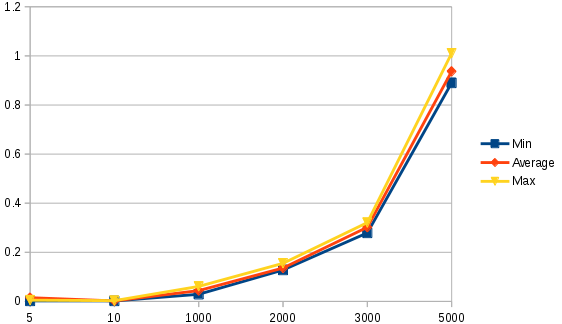
\includegraphics[scale=0.6]{rapport/avg_comp_iter_graph.png}
			\caption{Temps d'exécution minimum, moyen et maximum en fonction du nombre de noeud}
		\end{center}
	\end{figure}

\subsection{Analyse des résultats expérimentaux}
{ On obtient des résultats cohérents avec notre analyse théorique lors des test expérimentaux.\\
  Malgré notre implémentation peu optimale en terme d'utilisation du cache, le pourcentage de cache miss est assez faible.
}

\end{document}
%% Fin mise au format

